\documentclass[10pt,a4paper]{article}
\usepackage[margin=1.1cm,top=1.2cm,bottom=1.2cm]{geometry}
\usepackage{amsmath,amssymb,amsfonts}
\usepackage{tcolorbox}
\tcbuselibrary{skins,breakable}
\usepackage{booktabs}
\usepackage{tabularx}
\usepackage{colortbl}
\usepackage{xcolor}
\usepackage{enumitem}
\usepackage{graphicx}
\usepackage{titlesec}
\usepackage{microtype}
\usepackage{fancyhdr}

% Course Color Palette
\definecolor{themeblue}{HTML}{2B5A87}
\definecolor{lightbg}{HTML}{E8EEF4}
\definecolor{accentred}{HTML}{C8453A}
\definecolor{accentgreen}{HTML}{2E7D32}
\definecolor{darkgray}{HTML}{333333}
\definecolor{lightgray}{HTML}{D0D8E0}

% Header and Footer
\pagestyle{fancy}
\fancyhf{}
\renewcommand{\headrulewidth}{0.4pt}
\renewcommand{\footrulewidth}{0.4pt}
\fancyhead[L]{\footnotesize\bfseries\color{themeblue} Deep Learning Summary --- Lecture 8: Neural Networks 3}
\fancyhead[R]{\footnotesize\color{darkgray} ENSIA 2026--2027}
\fancyfoot[L]{\footnotesize\color{darkgray} Sid-Ahmed Berrani}
\fancyfoot[R]{\footnotesize\color{themeblue}\bfseries Page \thepage}

\begin{document}

% Title Banner
\begin{center}
    \vspace{-4pt}
    {\LARGE\bfseries\color{themeblue} Deep Learning: Neural Networks 3}\\[1.5pt]
    {\normalsize\bfseries Optimization Algorithms, Loss Landscapes, Multi-Class Softmax, and Batch Normalization}\\[2pt]
    {\footnotesize\color{darkgray} ENSIA 2026--2027 \quad$\vert$\quad Instructor: Prof. Sid-Ahmed Berrani}
\end{center}

\vspace{-8pt}

% =========================================================================
% PAGE 1: Mini-Batch Gradient Descent & Optimization Challenges
% =========================================================================

\noindent{\large\bfseries\color{themeblue} 1. Mini-Batch Gradient Descent \& Loss Landscapes}\par\vspace{1pt}
Training deep neural networks on massive datasets ($m = 10^6 - 10^8$) is computationally expensive. We accelerate training by dividing the dataset into smaller, manageable chunks called \textbf{mini-batches}.

\begin{itemize}[leftmargin=10pt, itemsep=1pt, topsep=0.5pt]
    \item \textbf{Batch Gradient Descent (Size = $m$):} Processes all $m$ training examples before making a single parameter update. Descent is smooth and monotonic, but agonizingly slow per step on large datasets.
    \item \textbf{Stochastic Gradient Descent (Size = 1):} Updates weights after every single example. Fast updates, but extremely noisy and erratic; never truly converges, and loses GPU matrix parallelization.
    \item \textbf{Mini-Batch Gradient Descent ($1 < \text{Size} < m$):} The ideal balance: vectorization speedup on GPU/CPU + frequent parameter updates per epoch.
    \item \textbf{Definition of an Epoch:} One complete pass through the entire training set of $m$ examples.
\end{itemize}

\vspace{-4pt}

\begin{center}
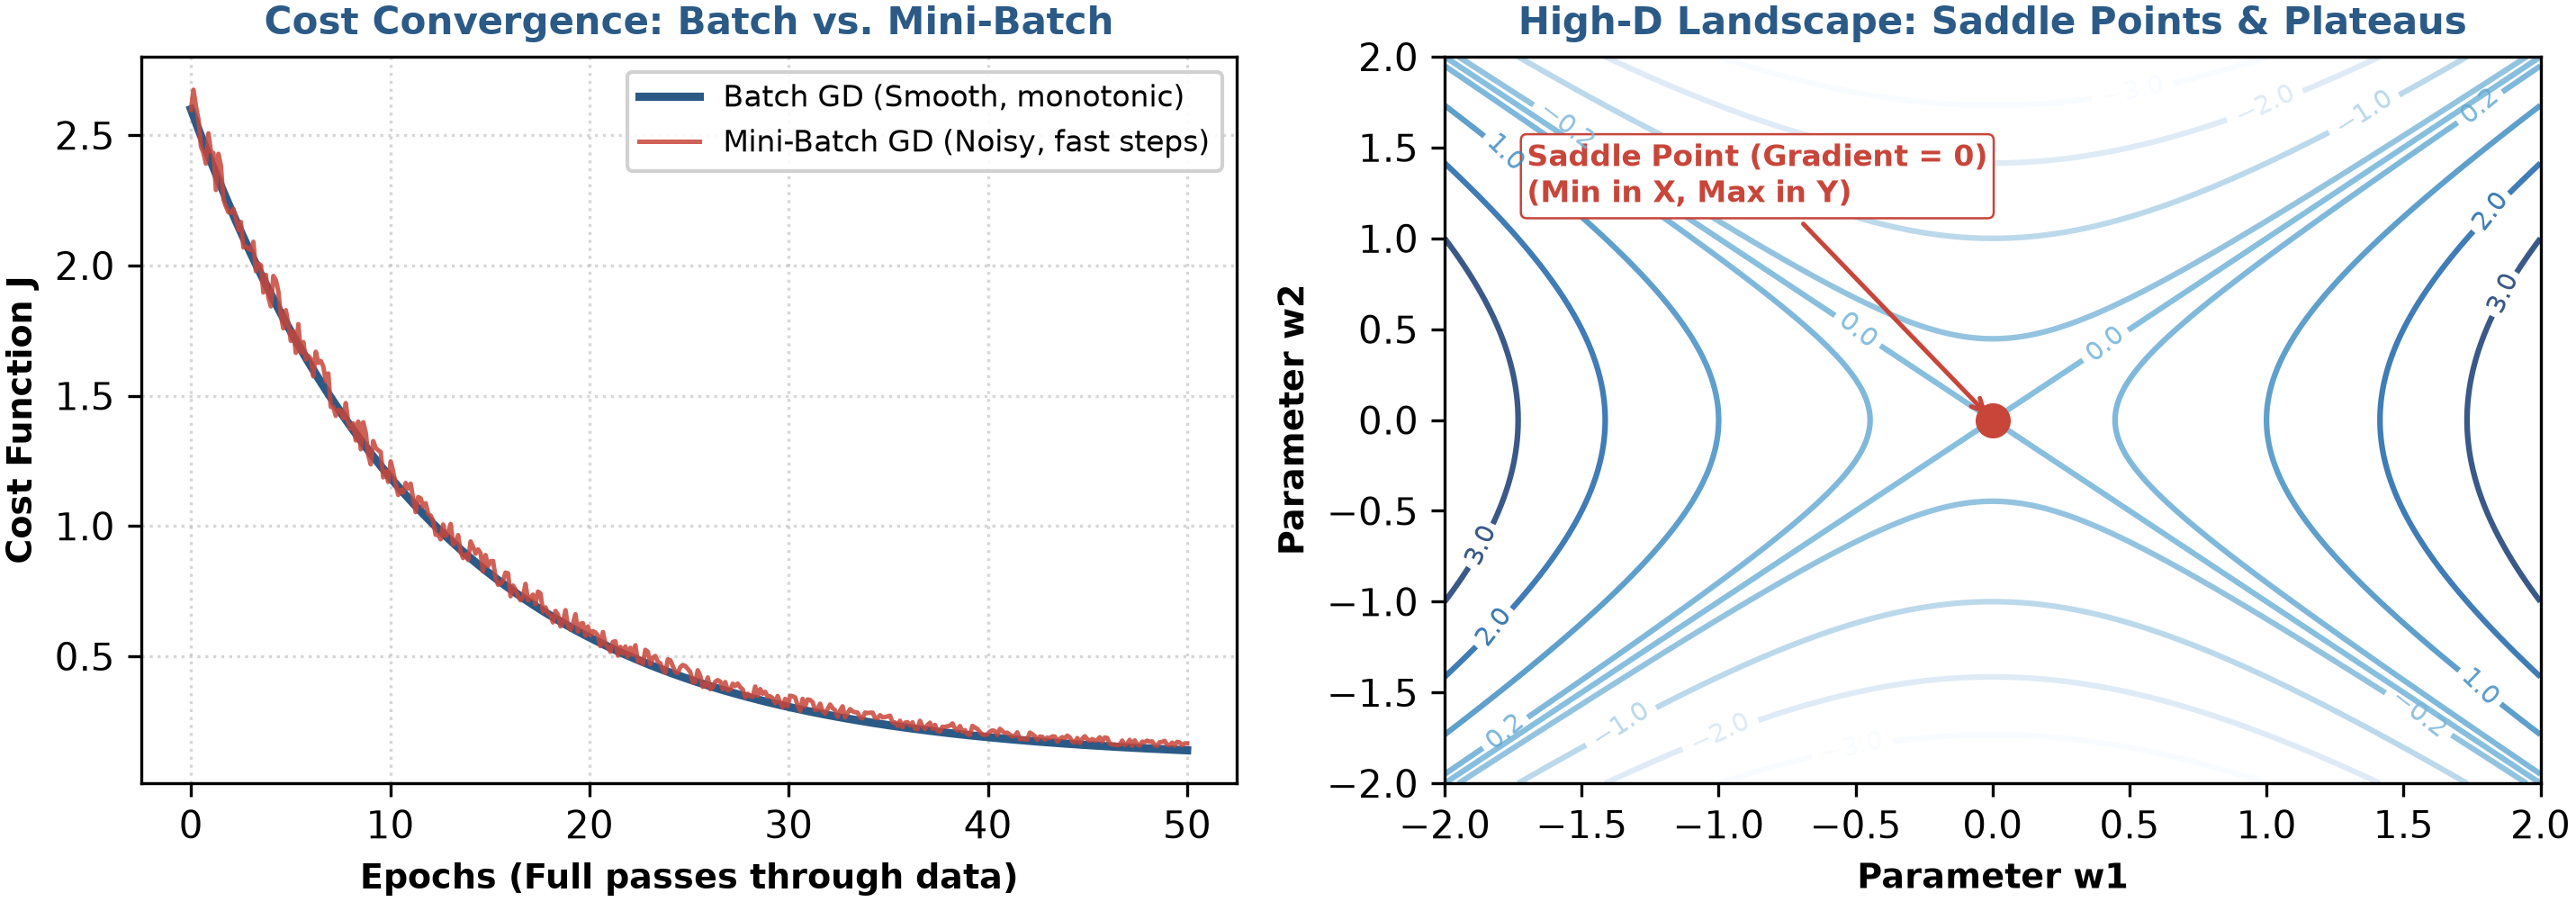
\includegraphics[width=0.82\textwidth]{nn3_minibatch_landscapes.png}\\[-1pt]
{\footnotesize\textit{Left: Cost curve comparison (Batch vs. Mini-Batch). Right: Saddle points and flat plateaus dominate high-dimensional landscapes.}}
\end{center}

\vspace{-6pt}

% Mini-batch sizing rules box
\begin{tcolorbox}[
    colframe=themeblue, colback=lightbg, coltitle=white,
    fonttitle=\bfseries\sffamily\small,
    title={Practical Rules for Mini-Batch Sizing},
    arc=1.3mm, boxrule=0.5pt, left=5pt, right=5pt, top=2pt, bottom=2pt
]
\footnotesize
The mini-batch size is an important hyperparameter:
\begin{itemize}[leftmargin=8pt, itemsep=1pt, topsep=0pt]
    \item \textbf{Small Datasets ($m < 2000$):} Use standard \textbf{Batch Gradient Descent} (batch size $= m$). Memory overhead is trivial and convergence is smooth.
    \item \textbf{Large Datasets ($m \ge 2000$):} Use mini-batch sizes that are \textbf{powers of 2}:
    \[
    \text{Batch Size} \in \{64, \; 128, \; 256, \; 512, \; 1024\}
    \]
    \item \textbf{Hardware Alignment:} Powers of 2 match CPU/GPU memory architecture, maximizing cache efficiency and SIMD tensor core utilization.
    \item \textbf{Memory Constraint:} Ensure that all input features and activations for a full mini-batch comfortably fit within CPU/GPU RAM.
\end{itemize}
\end{tcolorbox}

\vspace{-2pt}

% Loss Landscape & EWA Box
\begin{tcolorbox}[
    colframe=accentred, colback=white, arc=1.3mm, boxrule=0.5pt,
    left=5pt, right=5pt, top=2pt, bottom=2pt
]
\footnotesize
\textbf{Optimization Challenges in High-Dimensional Loss Landscapes:}
\begin{itemize}[leftmargin=8pt, itemsep=1pt, topsep=0pt]
    \item \textbf{The Local Minima Myth:} In high dimensions ($10^5$ to $10^8$ weights), the probability that all directions simultaneously slope upwards is virtually zero. Almost all zero-gradient critical points are \textbf{Saddle Points} (local minimum in some directions, local maximum in others).
    \item \textbf{Flat Plateaus:} Saddle points are surrounded by wide regions where gradients are nearly zero ($\nabla J \approx 0$). Gradient descent slows down to a crawl in these regions.
    \item \textbf{Pathological Curvature (Ravines):} The loss surface forms an elongated valley with steep walls and a flat floor. Gradient descent oscillates violently back and forth between the walls rather than making progress along the floor.
\end{itemize}
\hrulefill\\[1pt]
\textbf{The Mathematical Foundation: Exponentially Weighted Averages (EWA):}
Used to track trends and smooth noisy sequences ($V_t = \beta V_{t-1} + (1 - \beta) \theta_t$ with $V_0 = 0$).
\[
V_t \approx \text{Average over the past } \mathbf{\frac{1}{1 - \beta}} \text{ steps} \qquad \Big(\beta = 0.9 \implies \approx 10 \text{ steps}; \quad \beta = 0.98 \implies \approx 50 \text{ steps}\Big)
\]
\end{tcolorbox}

\newpage

% =========================================================================
% PAGE 2: Advanced Optimizers (Momentum, RMSProp, Adam)
% =========================================================================

\noindent{\large\bfseries\color{themeblue} 2. Advanced Optimization Algorithms: Momentum, RMSProp, and Adam}\par\vspace{1pt}
Standard Gradient Descent suffers from violent oscillations along steep directions and excruciatingly slow progress along shallow directions. Modern adaptive optimizers solve this by utilizing gradient history.

\vspace{-2pt}

\begin{center}
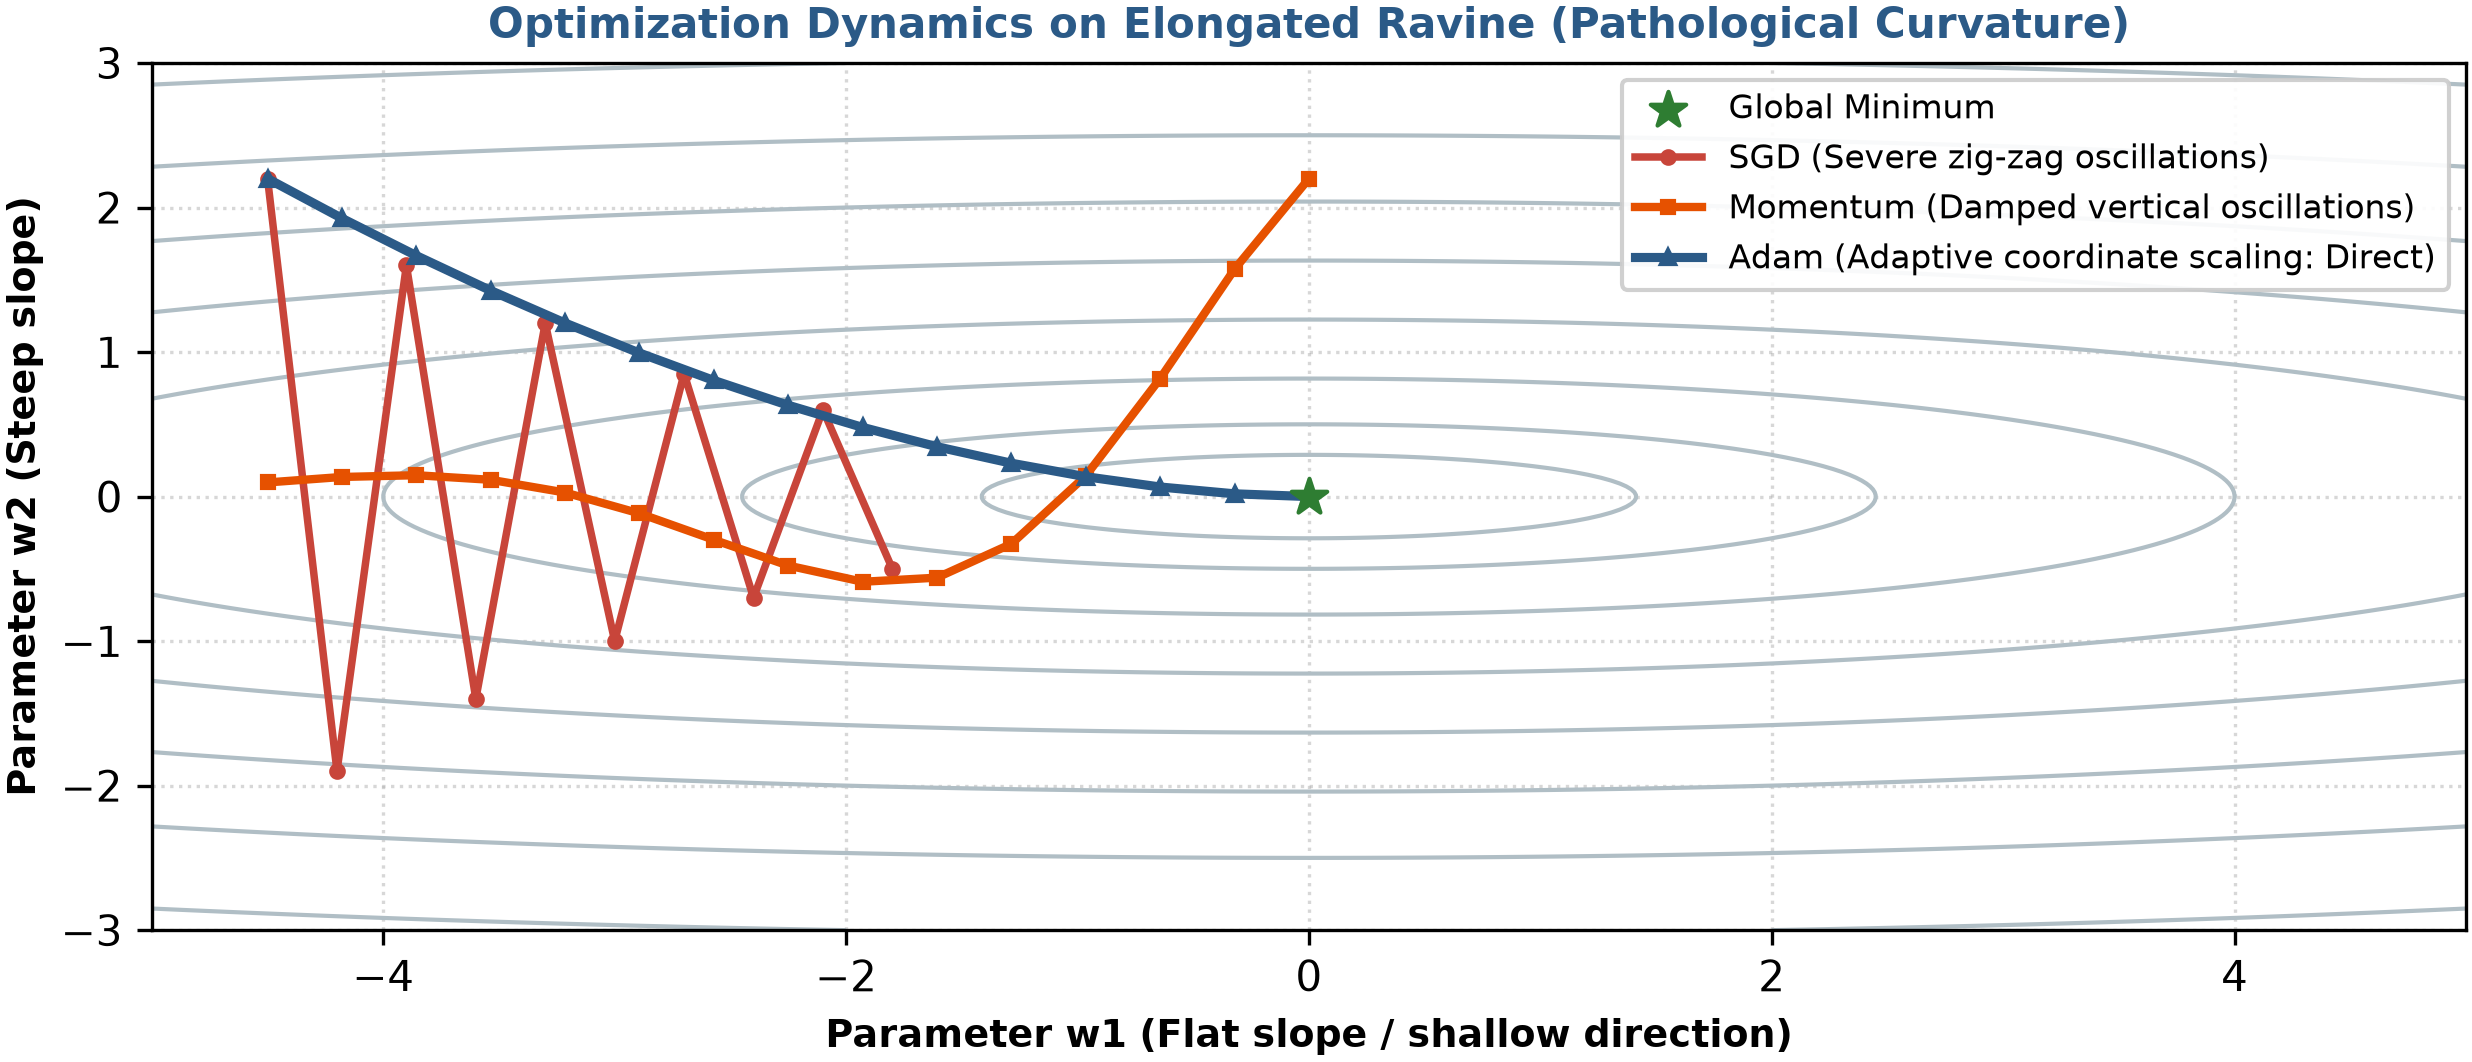
\includegraphics[width=0.78\textwidth]{nn3_optimizers_contours.png}\\[-1pt]
{\footnotesize\textit{Optimization paths on an elongated ravine: SGD oscillates wildly; Momentum cancels oscillations; Adam drives straight to the minimum.}}
\end{center}

\vspace{-6pt}

% Momentum Box
\begin{tcolorbox}[
    colframe=themeblue, colback=lightbg, coltitle=white,
    fonttitle=\bfseries\sffamily\small,
    title={1. Gradient Descent with Momentum (Adds Inertia)},
    arc=1.3mm, boxrule=0.5pt, left=5pt, right=5pt, top=2pt, bottom=2pt
]
\footnotesize
\textbf{Core Concept:} Computes an exponentially weighted average of past gradients and uses this ``velocity'' $v$ to update parameters. Acts like a heavy ball rolling down a ravine:
\begin{align*}
v_{dw} &= \beta v_{dw} + (1 - \beta) dw, \qquad v_{db} = \beta v_{db} + (1 - \beta) db \\[1.5pt]
w &:= w - \alpha v_{dw}, \qquad\qquad\quad\; b := b - \alpha v_{db} \qquad\qquad (\text{Default } \beta = 0.9)
\end{align*}
\textbf{Key Benefits:}
\begin{itemize}[leftmargin=8pt, itemsep=0.5pt, topsep=0pt]
    \item \textbf{Cancels Oscillations:} Across vertical walls, alternating positive and negative gradients average out to zero. Along the valley floor, persistent gradients accumulate, accelerating descent.
    \item \textbf{Escapes Vanishing Gradients \& Plateaus:} When current gradient $dw \approx 0$, momentum carries updates forward ($v \approx \beta v > 0$), coasting through flat plateaus!
\end{itemize}
\end{tcolorbox}

\vspace{-2pt}

% RMSProp Box
\begin{tcolorbox}[
    colframe=accentred, colback=white, coltitle=white,
    fonttitle=\bfseries\sffamily\small,
    title={2. RMSProp: Root Mean Square Propagation (Geoffrey Hinton)},
    arc=1.3mm, boxrule=0.5pt, left=5pt, right=5pt, top=2pt, bottom=2pt
]
\footnotesize
\textbf{Core Concept:} Tracks the exponentially weighted average of \textbf{squared gradients} ($s$), and divides updates by $\sqrt{s}$:
\begin{align*}
s_{dw} &= \beta_2 s_{dw} + (1 - \beta_2) dw^2, \qquad s_{db} = \beta_2 s_{db} + (1 - \beta_2) db^2 \\[1.5pt]
w &:= w - \alpha \frac{dw}{\sqrt{s_{dw}} + \epsilon}, \qquad\qquad b := b - \alpha \frac{db}{\sqrt{s_{db}} + \epsilon} \qquad (\text{Default } \beta_2 = 0.999, \; \epsilon = 10^{-8})
\end{align*}
\textbf{Self-Tuning Coordinate Scaling:}
\begin{itemize}[leftmargin=8pt, itemsep=0.5pt, topsep=0pt]
    \item In steep, oscillating directions ($w_2$): gradients are large $\implies s_{dw}$ is large $\implies$ divides by large number $\implies$ \textbf{dampens oscillations}.
    \item In shallow, slow directions ($w_1$): gradients are tiny $\implies s_{dw}$ is small $\implies$ divides by small number $\implies$ \textbf{accelerates progress}.
\end{itemize}
\end{tcolorbox}

\vspace{-2pt}

% Adam Box
\begin{tcolorbox}[
    colframe=accentgreen, colback=white, coltitle=white,
    fonttitle=\bfseries\sffamily\small,
    title={3. Adam: Adaptive Moment Estimation (Kingma \& Ba 2015)},
    arc=1.3mm, boxrule=0.5pt, left=5pt, right=5pt, top=2pt, bottom=2pt
]
\footnotesize
\textbf{Core Concept:} Combines \textbf{Momentum} (1st moment, direction) with \textbf{RMSProp} (2nd moment, coordinate scaling), plus \textbf{Bias Correction} to fix early steps (since $v_0 = s_0 = 0$):
\begin{enumerate}[leftmargin=12pt, itemsep=1pt, topsep=0.5pt]
    \item \textbf{Update 1st \& 2nd Moments:} $v_{dw} = \beta_1 v_{dw} + (1 - \beta_1) dw, \quad s_{dw} = \beta_2 s_{dw} + (1 - \beta_2) dw^2$
    \item \textbf{Bias Correction (Crucial for early steps):} $v_{dw}^{\text{corr}} = \frac{v_{dw}}{1 - \beta_1^t}, \quad s_{dw}^{\text{corr}} = \frac{s_{dw}}{1 - \beta_2^t}$
    \item \textbf{Update Parameter:} $w := w - \alpha \frac{v_{dw}^{\text{corr}}}{\sqrt{s_{dw}^{\text{corr}}} + \epsilon} \qquad (\text{Defaults: } \beta_1 = 0.9, \; \beta_2 = 0.999, \; \epsilon = 10^{-8})$
\end{enumerate}
\end{tcolorbox}

\vspace{-2pt}

% Optimizer Comparison Table
\noindent{\bfseries\color{themeblue} Summary of Optimizers:}\par\vspace{1pt}
\begin{center}
\footnotesize
\setlength{\tabcolsep}{4pt}
\begin{tabularx}{\textwidth}{p{0.18\textwidth}p{0.32\textwidth}p{0.20\textwidth}>{\raggedright\arraybackslash}X}
\toprule
\rowcolor{lightbg}
\textbf{Optimizer} & \textbf{Update Formula} & \textbf{Key Hyperparameters} & \textbf{Primary Advantage} \\
\midrule
\textbf{SGD} & $w := w - \alpha dw$ & $\alpha$ & Baseline, high oscillation in ravines. \\
\midrule
\textbf{Momentum} & $v := \beta v + (1-\beta)dw; \ w := w - \alpha v$ & $\alpha, \; \beta = 0.9$ & Smooths noise; coasts through flat plateaus. \\
\midrule
\textbf{RMSProp} & $s := \beta_2 s + (1-\beta_2)dw^2; \ w := w - \alpha \frac{dw}{\sqrt{s}+\epsilon}$ & $\alpha, \; \beta_2 = 0.999, \; \epsilon = 10^{-8}$ & Per-parameter adaptive learning rate. \\
\midrule
\textbf{Adam} & Combines $v^{\text{corr}}$ and $\sqrt{s^{\text{corr}}}$ & $\alpha, \; \beta_1 = 0.9, \; \beta_2 = 0.999$ & \textbf{De facto industry standard}; fast, robust. \\
\bottomrule
\end{tabularx}
\end{center}

\newpage

% =========================================================================
% PAGE 3: Learning Rate Schedules & Multi-Class Softmax Classification
% =========================================================================

\noindent{\large\bfseries\color{themeblue} 3. Learning Rate Decay \& Multi-Class Softmax Classification}\par\vspace{1pt}
A fixed learning rate $\alpha$ is suboptimal: we need large steps early on to traverse parameter space, but small steps later to settle cleanly into the minimum without oscillating around it.

\begin{itemize}[leftmargin=10pt, itemsep=1pt, topsep=0.5pt]
    \item \textbf{Early Training:} The model is far from the minimum $\implies$ large learning rate $\alpha$ enables fast progress.
    \item \textbf{Late Training:} Near the minimum, a fixed $\alpha$ causes the optimizer to bounce around the basin without converging. Decaying $\alpha$ allows tight, fine-tuned convergence.
\end{itemize}

\vspace{-4pt}

\begin{center}
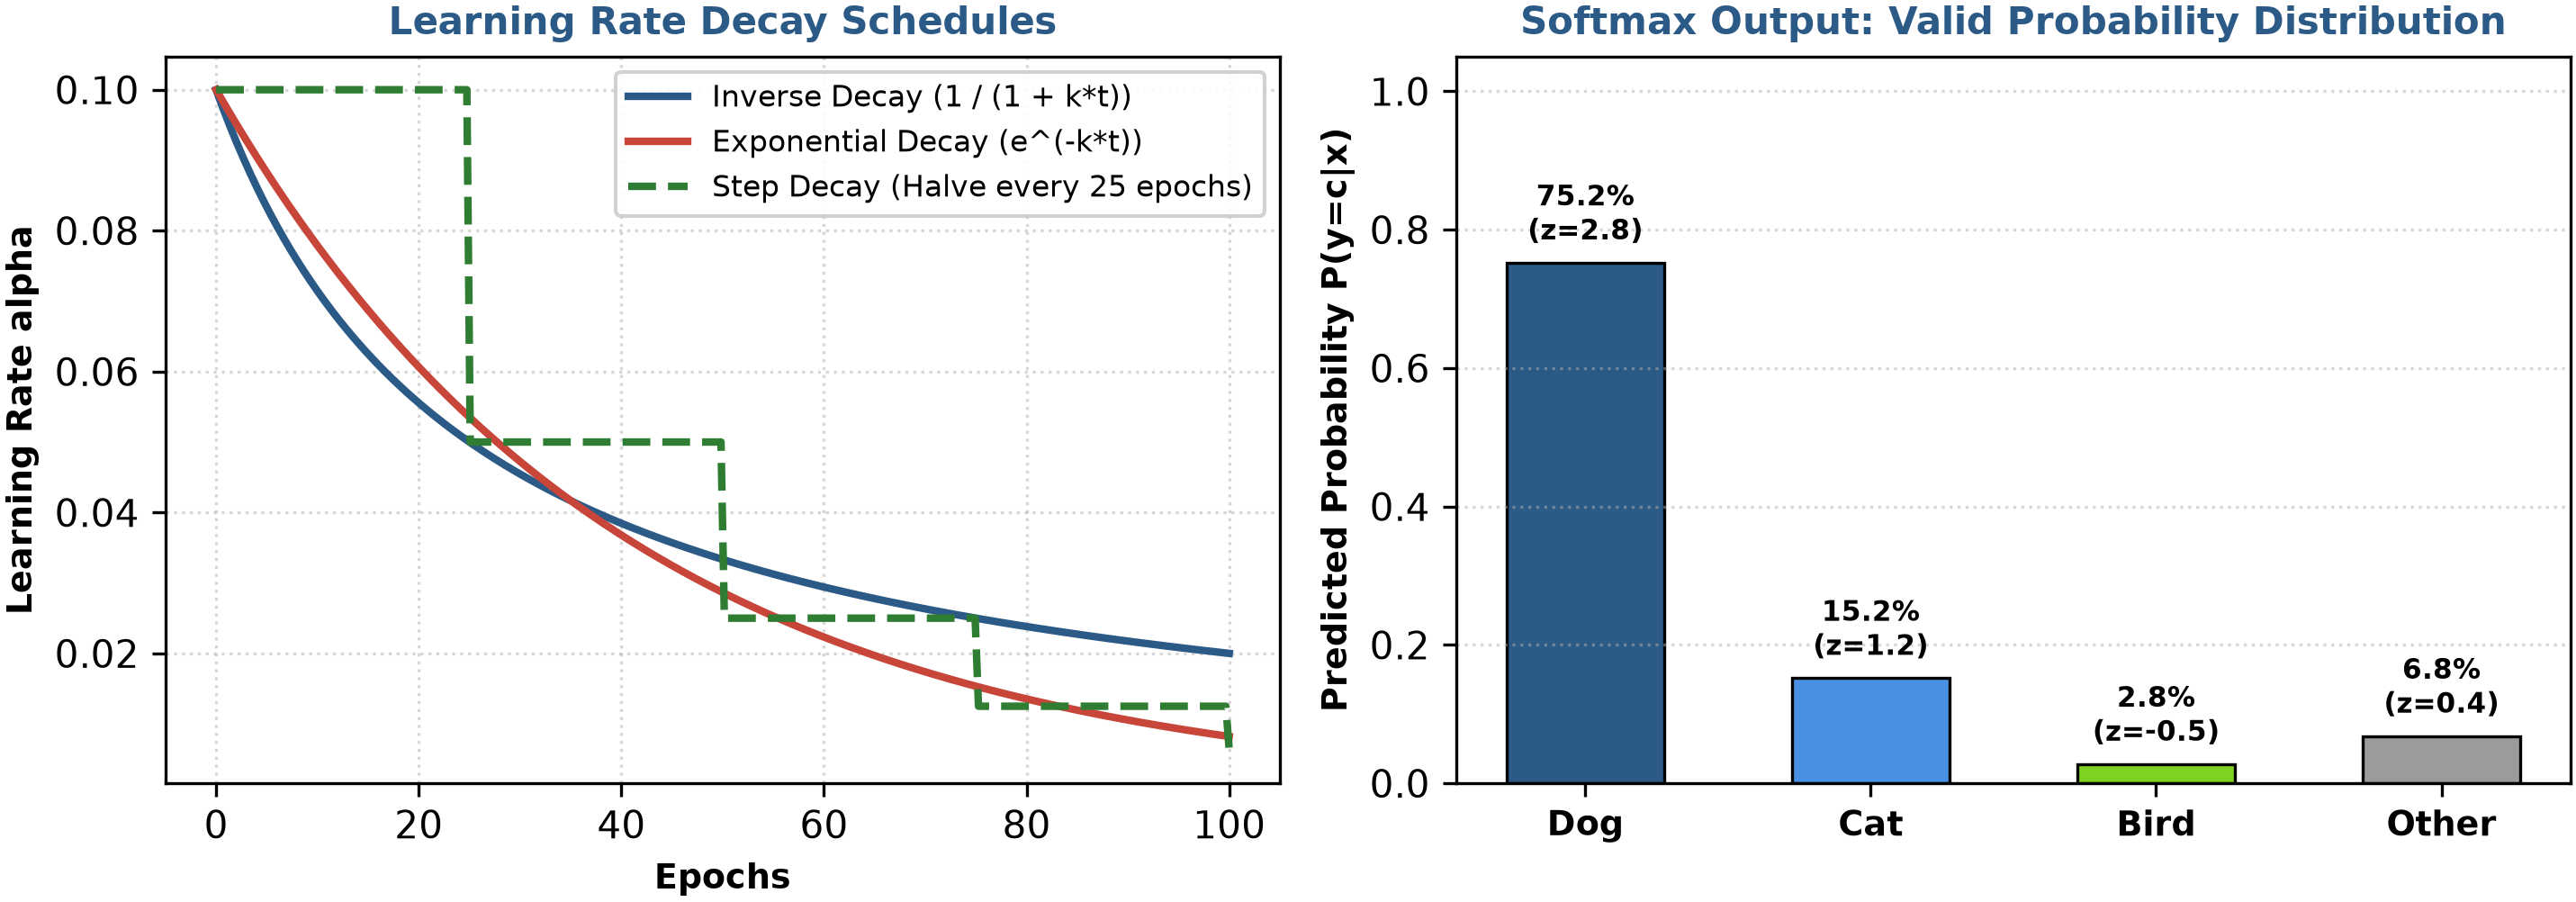
\includegraphics[width=0.82\textwidth]{nn3_softmax_decay.png}\\[-1pt]
{\footnotesize\textit{Left: Learning rate decay schedules. Right: Softmax maps linear logits $z$ into a normalized probability distribution.}}
\end{center}

\vspace{-6pt}

% Learning Rate Decay Schedules Box
\begin{tcolorbox}[
    colframe=themeblue, colback=lightbg, coltitle=white,
    fonttitle=\bfseries\sffamily\small,
    title={Common Learning Rate Decay Schedules (Epoch $t+1$)},
    arc=1.3mm, boxrule=0.5pt, left=5pt, right=5pt, top=2pt, bottom=2pt
]
\footnotesize
Where $t+1$ is the current epoch number, $\alpha_t$ is the previous epoch's learning rate, and $k$ is a hyperparameter:
\begin{itemize}[leftmargin=10pt, itemsep=1pt, topsep=0pt]
    \item \textbf{Default (Inverse Decay):} $\alpha_{t+1} = \frac{1}{1 + k \cdot t} \cdot \alpha_t$ \quad (smooth, gradual decay).
    \item \textbf{Step Decay:} Drops the learning rate by a fixed factor every few epochs (e.g., typically halve $\alpha$ every 10 epochs).
    \item \textbf{Discrete Staircase:} $\alpha_{t+1} = \frac{k}{\sqrt{t}} \cdot \alpha_t$ \quad (inversely proportional to $\sqrt{t}$).
    \item \textbf{Exponential Decay:} $\alpha_{t+1} = \alpha_t \cdot e^{-k \cdot t}$ \quad (faster, sharper drop-off).
\end{itemize}
\end{tcolorbox}

\vspace{-2pt}

% Softmax & Categorical Cross Entropy Box
\begin{tcolorbox}[
    colframe=accentred, colback=white, coltitle=white,
    fonttitle=\bfseries\sffamily\small,
    title={Multi-Class Classification with Softmax Activation ($C > 2$ Classes)},
    arc=1.3mm, boxrule=0.5pt, left=5pt, right=5pt, top=2pt, bottom=2pt
]
\footnotesize
To classify inputs into $C$ mutually exclusive categories (e.g., Dog, Cat, Bird, Other), the output layer has $C$ neurons:
\begin{enumerate}[leftmargin=12pt, itemsep=1pt, topsep=0.5pt]
    \item \textbf{Linear Logits:} Compute output layer activations: $z^{[L]} = W^{[L]} a^{[L-1]} + b^{[L]} \in \mathbb{R}^C$.
    \item \textbf{Exponentiation:} $t_i = e^{z_i^{[L]}}$ (ensures all terms are strictly positive).
    \item \textbf{Softmax Normalization:} Divide each term by the sum of all exponentiated logits:
    \[
    a_i^{[L]} = \hat{y}_i = \frac{e^{z_i^{[L]}}}{\sum_{j=1}^C e^{z_j^{[L]}}} \qquad \text{for } i = 1, 2, \dots, C
    \]
\end{enumerate}
\hrulefill\\[1pt]
\textbf{Key Mathematical Properties of Softmax:}
\begin{itemize}[leftmargin=8pt, itemsep=0.5pt, topsep=0pt]
    \item Every predicted probability is strictly bounded: $0 < \hat{y}_i < 1$.
    \item The sum of all output probabilities is \textbf{guaranteed to be 1}: $\sum_{i=1}^C \hat{y}_i = 1$. It forms a valid probability distribution!
    \item If $C = 2$, Softmax is mathematically identical to the standard Sigmoid function.
\end{itemize}
\end{tcolorbox}

\vspace{-2pt}

% Categorical Cross-Entropy Box
\begin{tcolorbox}[
    colframe=themeblue, colback=lightbg, arc=1.3mm, boxrule=0.5pt,
    left=5pt, right=5pt, top=2pt, bottom=2pt
]
\footnotesize
\textbf{Categorical Cross-Entropy Loss Function:}
For ground truth vector $y \in \{0, 1\}^C$ (one-hot encoded) and prediction vector $\hat{y} \in (0, 1)^C$:
\[
\mathcal{L}(\hat{y}, y) = - \sum_{i=1}^C y_i \log(\hat{y}_i)
\]
\textbf{Loss Behavior on a One-Hot Target (Suppose True Class is $k$, so $y_k = 1$ and $y_{j \neq k} = 0$):}
\[
\mathcal{L}(\hat{y}, y) = - \log(\hat{y}_k)
\]
\begin{itemize}[leftmargin=8pt, itemsep=0.5pt, topsep=0pt]
    \item If model predicts $\hat{y}_k = 1$ (confident \& correct): $\mathcal{L} = -\log(1) = 0$ (Zero penalty).
    \item If model predicts $\hat{y}_k = 0.5$: $\mathcal{L} = -\log(0.5) \approx 0.693$.
    \item If model predicts $\hat{y}_k \to 0$ (completely wrong): $\mathcal{L} = -\log(0) \to +\infty$ (Infinite penalty!).
\end{itemize}
\end{tcolorbox}

\newpage

% =========================================================================
% PAGE 4: Batch Normalization (Subtle Overview) & Hyperparameters Reference
% =========================================================================

\noindent{\large\bfseries\color{themeblue} 4. Batch Normalization (Overview) \& Hyperparameters Reference}\par\vspace{1pt}
Just as we normalize input features $x$ to have zero mean and unit variance (speeding up training), \textbf{Batch Normalization} normalizes the linear logits $z^{[l]}$ inside hidden layers.

\vspace{-2pt}

\begin{center}
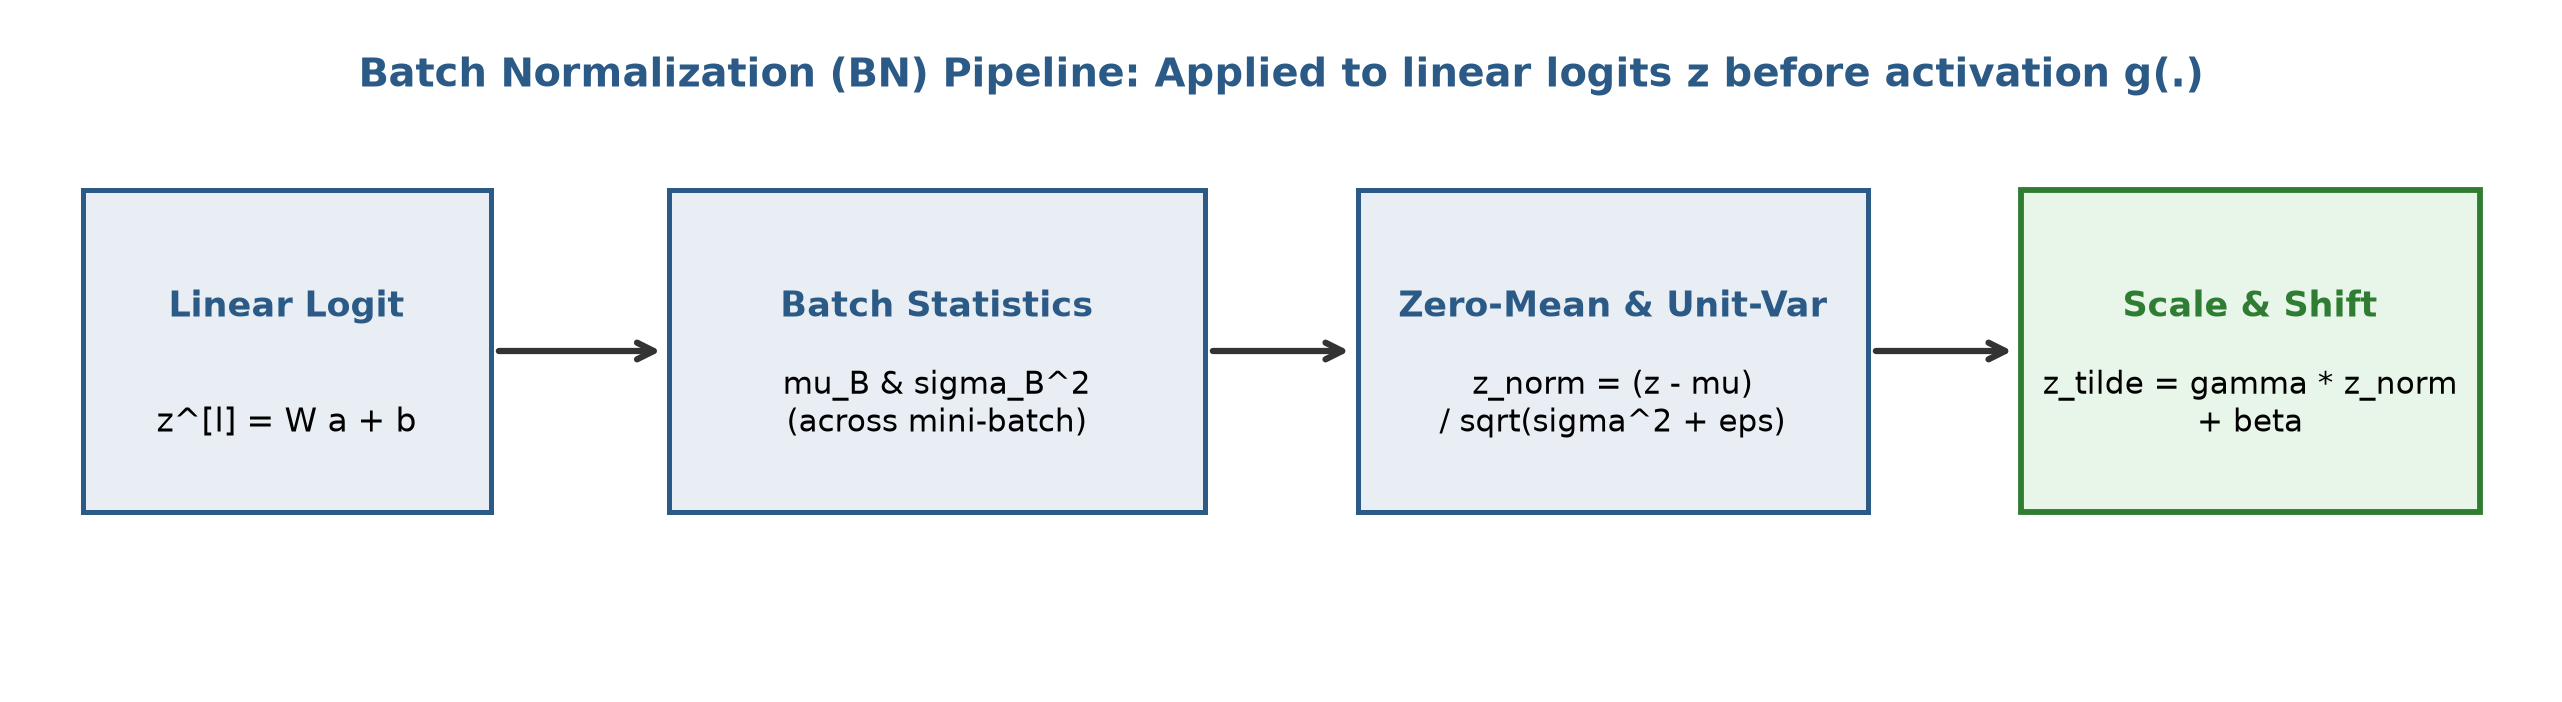
\includegraphics[width=0.80\textwidth]{nn3_batch_norm.png}\\[-1pt]
{\footnotesize\textit{Batch Normalization pipeline: Applied to linear logits $z^{[l]}$ across the mini-batch before applying activation $g(\tilde{z}^{[l]})$.}}
\end{center}

\vspace{-6pt}

% Batch Normalization 4-step box
\begin{tcolorbox}[
    colframe=themeblue, colback=lightbg, coltitle=white,
    fonttitle=\bfseries\sffamily\small,
    title={Batch Normalization in 4 Steps (Mini-Batch of size $m$)},
    arc=1.3mm, boxrule=0.5pt, left=5pt, right=5pt, top=2pt, bottom=2pt
]
\footnotesize
For a hidden layer $l$, given mini-batch linear values $z^{(1)}, z^{(2)}, \dots, z^{(m)}$:
\begin{enumerate}[leftmargin=12pt, itemsep=1.5pt, topsep=0.5pt]
    \item \textbf{Compute Mini-Batch Mean:} $\mu = \frac{1}{m} \sum_{i=1}^m z^{(i)}$
    \item \textbf{Compute Mini-Batch Variance:} $\sigma^2 = \frac{1}{m} \sum_{i=1}^m \big(z^{(i)} - \mu\big)^2$
    \item \textbf{Standardize (Zero Mean, Unit Variance):} $z_{\text{norm}}^{(i)} = \frac{z^{(i)} - \mu}{\sqrt{\sigma^2 + \epsilon}}$ \quad ($\epsilon \approx 10^{-8}$ avoids division by zero)
    \item \textbf{Scale and Shift (Learnable Parameters $\gamma$ and $\beta$):}
    \[
    \tilde{z}^{(i)} = \gamma \cdot z_{\text{norm}}^{(i)} + \beta \qquad \Longrightarrow \qquad a^{(i)} = g\big(\tilde{z}^{(i)}\big)
    \]
\end{enumerate}
\hrulefill\\[1pt]
\textbf{Why Include Learnable $\gamma$ and $\beta$?}
If a hidden layer strictly had zero mean and unit variance, activations like Tanh would be permanently locked in their linear regime! Learnable parameters $\gamma$ and $\beta$ allow the network to \textbf{choose the optimal variance and mean for each layer} (if the network sets $\gamma = \sqrt{\sigma^2+\epsilon}$ and $\beta = \mu$, it can completely undo the normalization if needed).
\end{tcolorbox}

\vspace{-2pt}

% BN Key Takeaways Box
\begin{tcolorbox}[
    colframe=accentgreen, colback=white, arc=1.3mm, boxrule=0.5pt,
    left=5pt, right=5pt, top=2pt, bottom=2pt
]
\footnotesize
\textbf{Key Takeaways About Batch Normalization:}
\begin{itemize}[leftmargin=8pt, itemsep=1pt, topsep=0pt]
    \item \textbf{Where applied:} Applied directly to $z^{[l]}$ \textbf{before} the activation function $g(\cdot)$ (or right after $W A + b$).
    \item \textbf{Reduces Internal Covariate Shift:} Keeps the distribution of hidden inputs stable even as earlier layers update weights, allowing much \textbf{higher learning rates} $\alpha$ and accelerating training.
    \item \textbf{Slight Regularization Effect:} Each mini-batch's mean and variance add slight stochastic noise to the activations (similar to dropout).
    \item \textbf{What to do at Test Time?} At test time, examples are evaluated one by one (no mini-batch). The model uses a \textbf{running Exponential Moving Average} of $\mu$ and $\sigma^2$ accumulated across mini-batches during training.
\end{itemize}
\end{tcolorbox}

\vspace{-2pt}

% Master Hyperparameters Table
\noindent{\bfseries\color{themeblue} Master Deep Learning Hyperparameters Checklist:}\par\vspace{1pt}
\begin{center}
\footnotesize
\setlength{\tabcolsep}{4pt}
\begin{tabularx}{\textwidth}{p{0.24\textwidth}p{0.24\textwidth}>{\raggedright\arraybackslash}X}
\toprule
\rowcolor{lightbg}
\textbf{Hyperparameter} & \textbf{Typical Default / Range} & \textbf{Practical Guidance} \\
\midrule
\textbf{Learning Rate $\alpha$} & $0.001, \; 0.01, \; 0.1$ & \textbf{Most important hyperparameter}; tune first using logarithmic search. \\
\midrule
\textbf{Momentum Factor $\beta_1$} & $0.9$ & Averages over last $\approx 10$ gradients; rarely needs tuning. \\
\midrule
\textbf{RMSProp Factor $\beta_2$} & $0.999$ & Averages over last $\approx 1000$ squared gradients; almost never changed. \\
\midrule
\textbf{Adam Epsilon $\epsilon$} & $10^{-8}$ & Prevents numerical division by zero; leave at default. \\
\midrule
\textbf{Mini-Batch Size} & $64, \; 128, \; 256, \; 512$ & Powers of 2 matching hardware; tune based on GPU memory. \\
\midrule
\textbf{Learning Rate Decay $k$} & Scheduled ($0.5$ every $K$ ep) & Decays $\alpha$ in late epochs to allow fine-tuned convergence. \\
\midrule
\textbf{Architecture ($L, n^{[l]}$)} & Problem dependent & Increase depth/width for high bias; regularize for high variance. \\
\midrule
\textbf{Regularization ($\lambda, kp$)} & $\lambda \approx 10^{-4}-10^{-2}, \; kp=0.5-0.8$ & Increase $\lambda$ or lower $kp$ strictly when facing overfitting. \\
\bottomrule
\end{tabularx}
\end{center}

\end{document}
